\documentclass[14pt]{beamer}
\usetheme{Madrid}
\usepackage[utf8]{inputenc}
\usepackage[spanish]{babel}
\usepackage{amsmath}
\usepackage{amsfonts}
\usepackage{amssymb}
\usepackage{graphicx}
\definecolor{UBCblue}{rgb}{50, 0.1, 0.1}

\usecolortheme[named=UBCblue]{structure}

\author[Campanería, Fernández, Fuentes]
{David Campanería Cisneros\\Pablo Adrian Fuentes González\\Dayron Fernández Acosta}
\title[Aplicación   HCVet]
{HCVet: Aplicación móvil para historia clínica veterinaria.}
%\setbeamercovered{transparent} 
%\setbeamertemplate{navigation symbols}{} 
\logo{
\includegraphics[height=1cm]{Images/clean_app_icon.png}} 
\institute[UH]
{\textbf{Tutores:}\\ José Alejandro Mesejo Chiong\\ José Luis Castañeda Lorenzo} 
%\date{} 
%\subject{} 
\begin{document}

\begin{frame}
\titlepage
\end{frame}



\begin{frame}
\frametitle{Temática}
\begin{block}{Temática}
Creación de una herramienta que permita gestionar los datos clínicos históricos de la condición de salud y los servicios que han recibido animales domésticos.

\end{block}

\end{frame}


\begin{frame}
\frametitle{Objetivos}
El desarrollo de la app debe tener en cuenta :
\begin{itemize}
\item Facilidad de uso
\item Almacenamiento de Datos y características de animales
\item Sistema de registro de usuarios
\item Almacenamiento de Historiales Clínicos
\item Compartimiento de Datos 
\item Trabajo Offline

\end{itemize}

\end{frame}


\begin{frame}
\frametitle{Estado del arte}
Similares de desarrollos en el tema:


\begin{columns}
\begin{column}{0.3\textwidth}
\begin{center}


\includegraphics[scale =0.3]{Images/RCM.jpg}\\
\caption{RCM}\
%\footnote{Web del Registro Cubano de Mascotas.}
\end{center}
\end{column}
\begin{column}{0.3\textwidth}
\begin{center}


\includegraphics[scale =0.12]{Images/BAC.jpg}\\
\caption{BACuba}
\end{center}
\end{column}

\begin{column}{0.3\textwidth}
\begin{center}

\includegraphics[scale =0.13]{Images/DogH.png}\\
\caption{Dog Health}
\end{center}
\end{column}
\end{columns}

\end{frame}


\begin{frame}
\frametitle{Historia Clínica Veterinaria}

\begin{columns}
\begin{column}{0.5\textwidth}
\begin{center}

\fbox{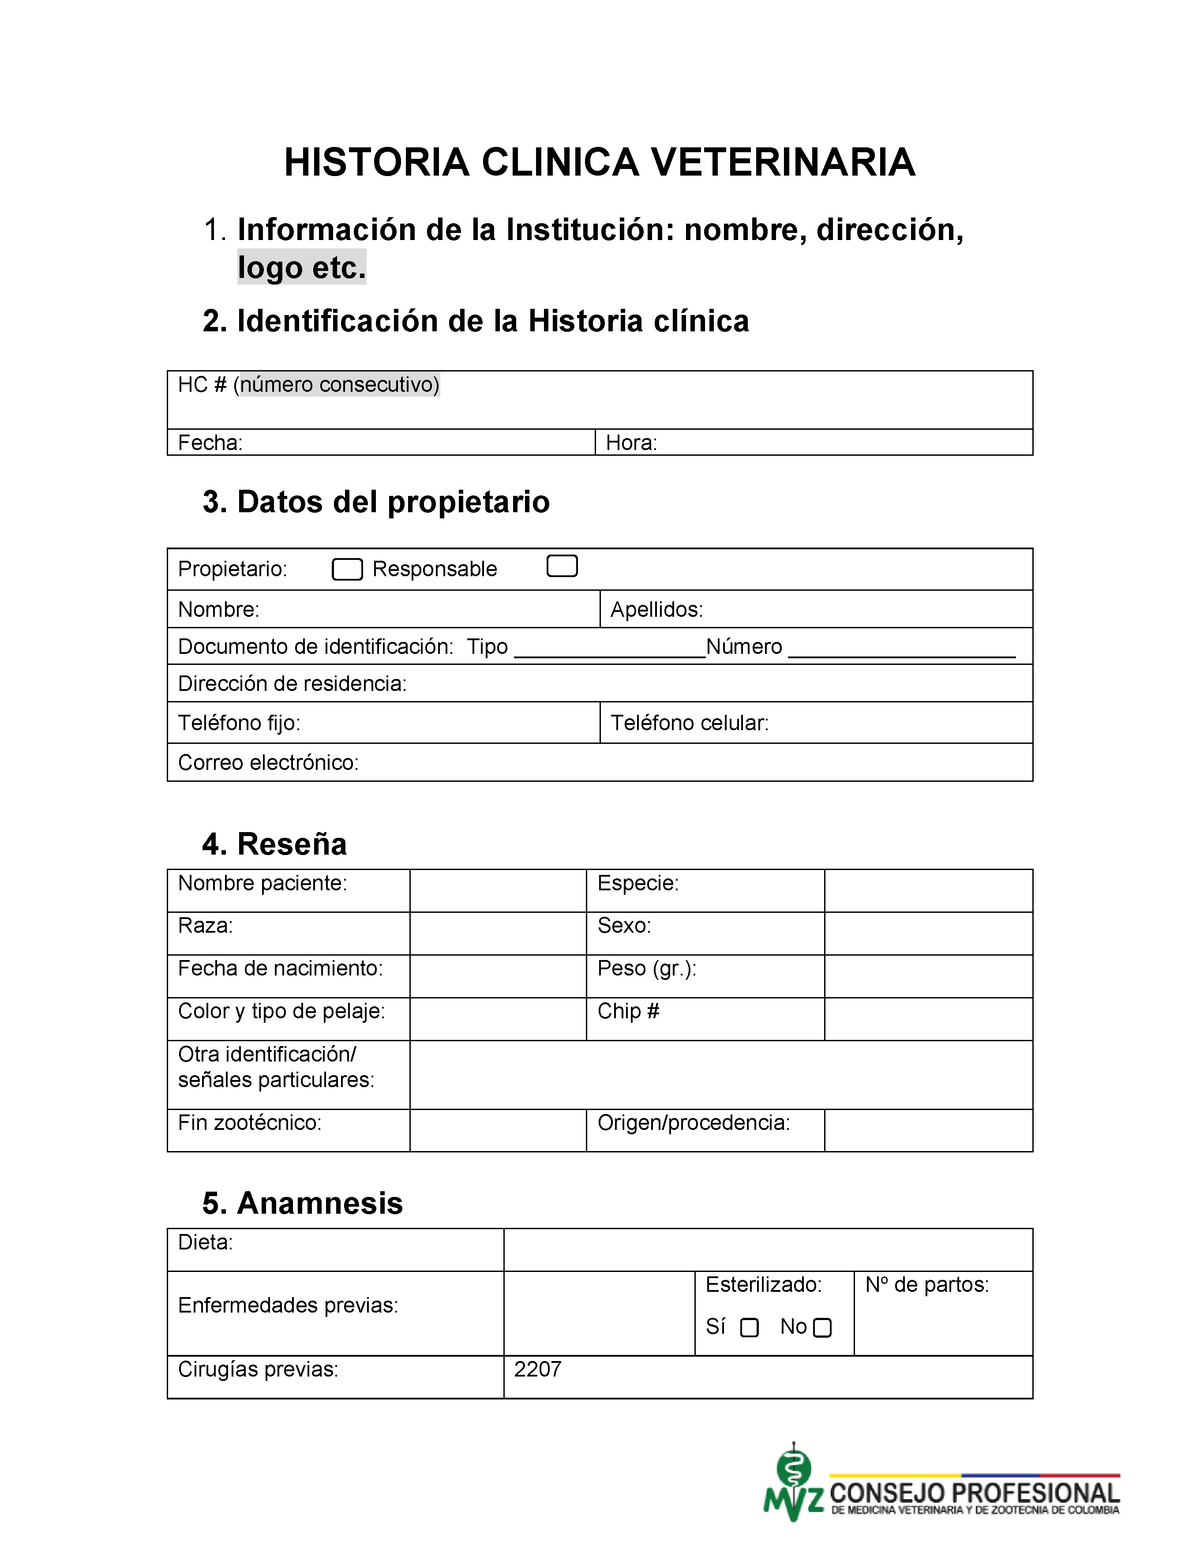
\includegraphics[scale =0.5]{Images/HC1.png}}

\end{center}
\end{column}
\begin{column}{0.5\textwidth}
\begin{center}

\fbox{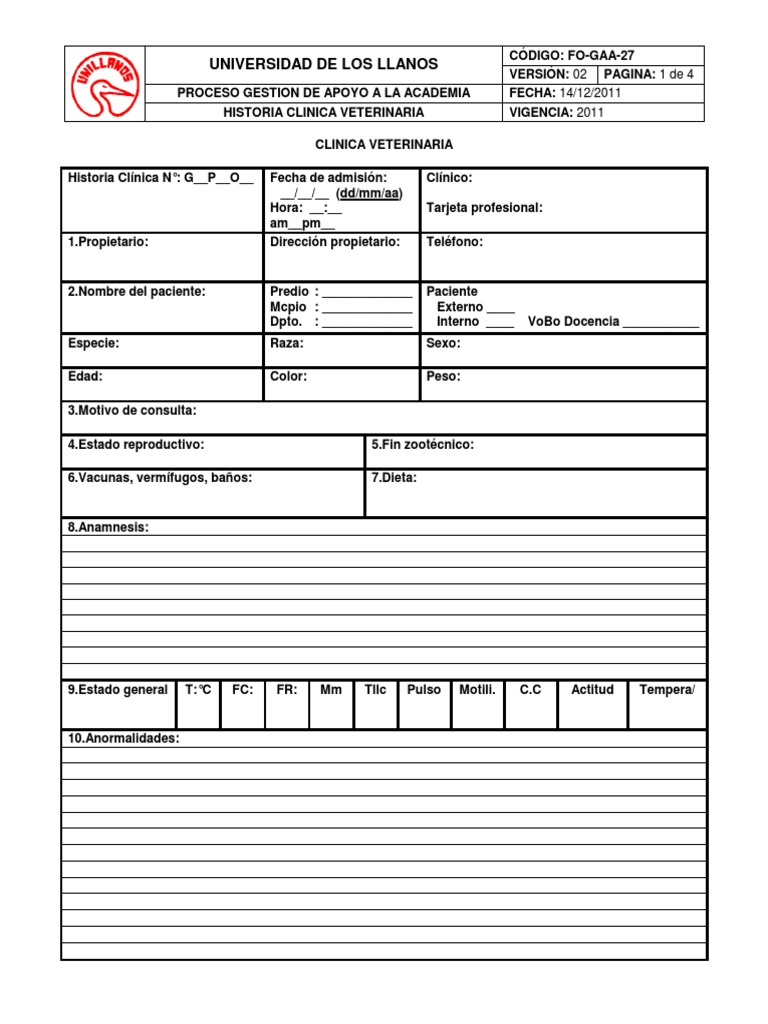
\includegraphics[scale =0.17]{Images/HC2.jpg}}

\end{center}
\end{column}
\end{columns}



\end{frame}


\begin{frame}
\frametitle{Importancia del problema}
Razones por las que son necesarias resolver el problema:
\begin{itemize}
\item Gran cantidad de datos
\item Poca agilidad del sistema actual
\item Datos difícilmente transferibles
\item Inconsistencia de los Datos
\end{itemize}

\end{frame}

\begin{frame}
\frametitle{Funcionalidades de la aplicación}
\begin{itemize}
\item Creación de una mascota
\item Eliminar mascota
\item Transferir una mascota a otro usuario de manera local.
\item Insertar nueva consulta
\item Insertar notas extras
\item Visualización

\end{itemize}

\end{frame}


\begin{frame}
\frametitle{Tecnologías utilizadas}

Tecnologías utilizadas:



\begin{columns}
\begin{column}{0.3\textwidth}
\begin{center}


\includegraphics[scale =0.45]{Images/LogodeFlutter.jpg}\\
\caption{Flutter}\
%\footnote{Web del Registro Cubano de Mascotas.}
\end{center}
\end{column}
\begin{column}{0.3\textwidth}
\begin{center}


\includegraphics[scale =0.10]{Images/LogoKotlin.jpg}\\
\caption{Kotlin}
\end{center}
\end{column}

\begin{column}{0.3\textwidth}
\begin{center}

\includegraphics[scale =0.08]{Images/LogodeSQLite.png}\\
\caption{SQLite}
\end{center}
\end{column}
\end{columns}


\end{frame}


\begin{frame}
\frametitle{Patrón Arquitectónico}

Fue utilizado un patrón \textbf{Model-View-ViewModel}.
\\
Componentes:
\begin{itemize}
\item Model
\item View
\item ViewModel
\end{itemize}

\begin{center}

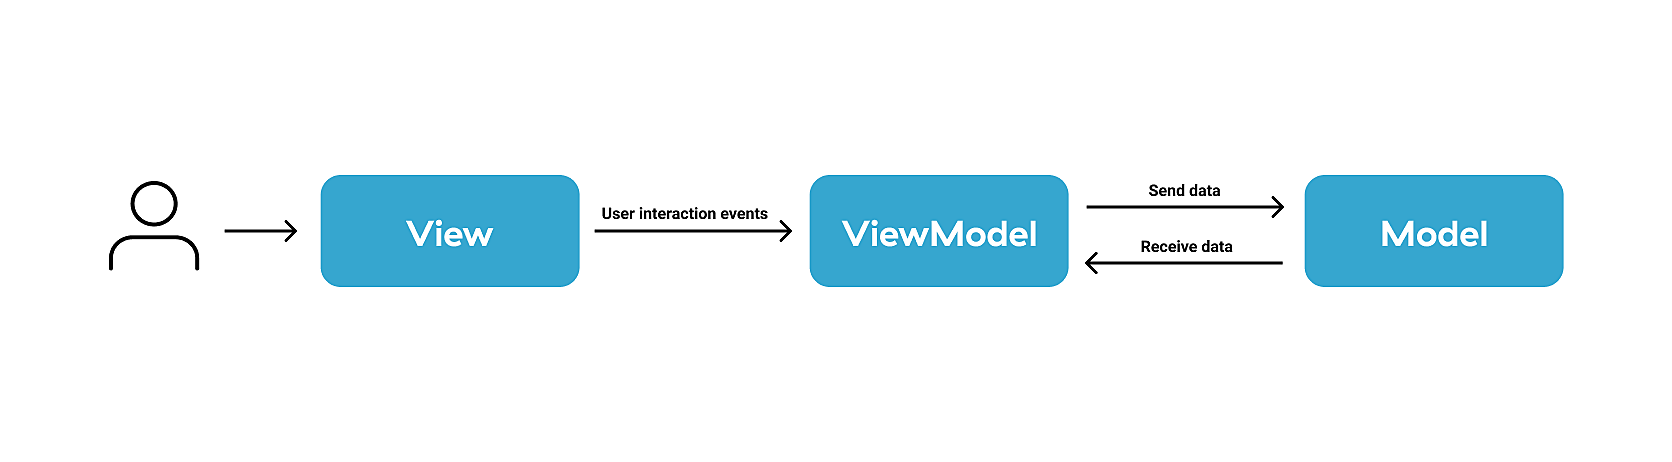
\includegraphics[scale =0.2]{Images/MVVMwip.png}


\end{center}

\end{frame}





\begin{frame}
\frametitle{Estructura de Model}

El Model está dividido en tres componentes principales:

\begin{itemize}
\item Componente de comunicación con el servidor (Online)

\item Componente de transferencia de datos no sincronizada sin conexión a internet. (Offline)

\item Componente de almacenamiento interno (Database)

\end{itemize}


\end{frame}

\begin{frame}
\frametitle{Componente de comunicación con el servidor.}

\begin{block}{}
Se establece comunicación con el servidor a través del protocolo HTTPS.
Este protocolo fue elegido gracias a que se priorizó la seguridad de los datos en la comunicación con el servidor.
\end{block}

\\
\\
Biblioteca: \textbf{http}(Pub.dev)
\end{frame}

\begin{frame}
\frametitle{Componente de transferencia de datos offline.}

\begin{block}{}
En la implementación de este componente fue utilizado Kotlin para hacer uso del API WifiP2pManager de Android.

Las bibliotecas de Flutter para el manejo de conexiones vía Wifi entre dispositivos están restringidos para SDK de Android mayor o igual que 26.
\end{block}

\end{frame}

\begin{frame}
\frametitle{Componente de almacenamiento interno.}

\textbf{Algunos de los métodos proporcionados por el paquete sqflite para el manejo de base de datos SQLite:}

\begin{itemize}


\item execute(...)
\item insert(...)
\item update(...)
\item query(...)
\item delete(...)
\end{itemize}

\end{frame}



\begin{frame}
\frametitle{Modelo de Datos}

\begin{center}

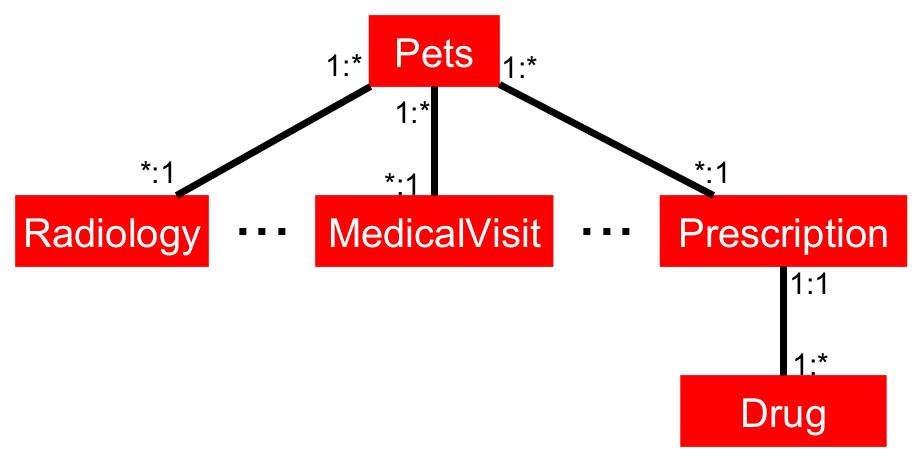
\includegraphics[scale =0.35]{Images/symplifiedClass.jpg}

\end{center}


\end{frame}


\begin{frame}
\frametitle{Estructura de View}
Los 5 principios utilizados para el diseño de la interfaz:
\begin{itemize}
\item Simplicidad
\item Eficiencia
\item Consistencia
\item Retroalimentación (Feedback)
\item Accesibilidad
\end{itemize}

\end{frame}

\begin{frame}
\frametitle{Estructura de View}
Las dos aproximaciones utilizadas para el diseño:

\begin{columns}
\begin{column}{0.5\textwidth}
\textbf{Menu-driven interface}
\begin{center}

\fbox{
\includegraphics[scale = 0.12]{Images/homePage.jpg}}

\end{center}
\end{column}
\begin{column}{0.5\textwidth}
\textbf{Form-based interface}
\begin{center}

\fbox{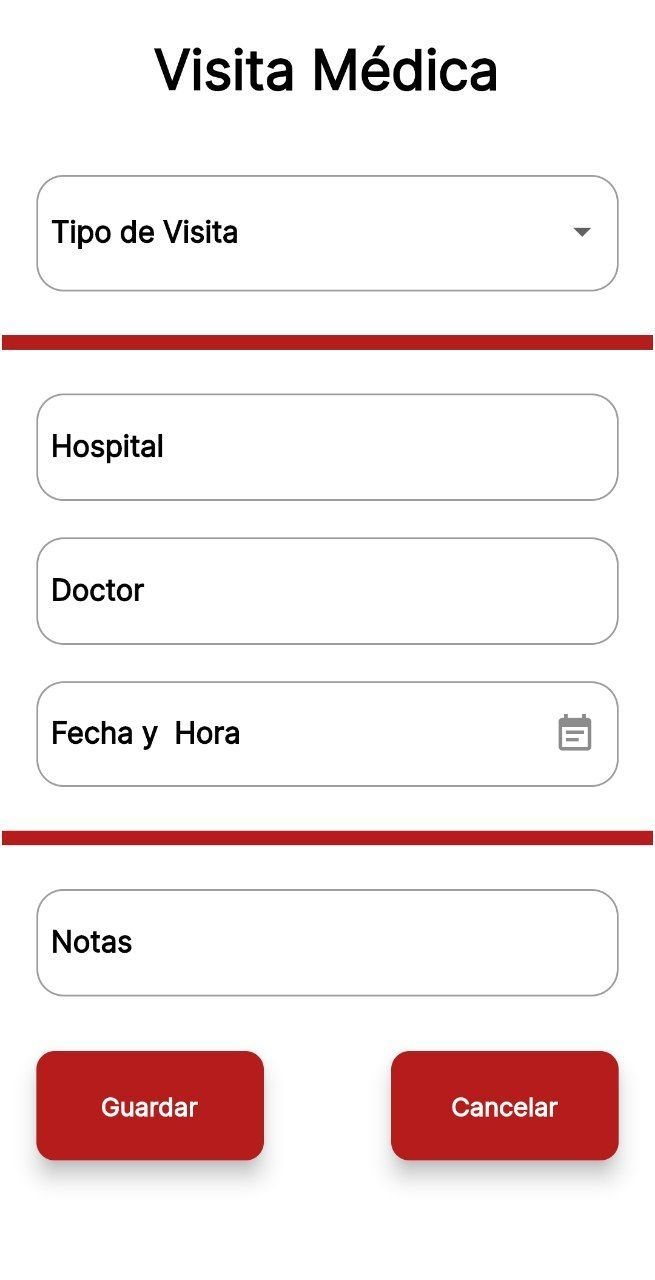
\includegraphics[scale = 0.12]{Images/form.jpg}}

\end{center}
\end{column}
\end{columns}

\end{frame}


\begin{frame}
\frametitle{Estructura de View-Model}
Componentes del View-Model:
\begin{itemize}
\item SyncroVM
\item KotlinChannelVM
\item DataBaseVM


\end{itemize}


\end{frame}


\begin{frame}
\frametitle{Aplicación: Registro y Autenticación}
\begin{columns}
\begin{column}{0.25\textwidth}
\begin{center}

\fbox{
\includegraphics[scale = 0.1]{Images/init.jpg}}
\begin{small}
\caption{Página Inicial de la Aplicación}
\end{small}
\end{center}
\end{column}

\begin{column}{0.25\textwidth}
\begin{center}

\fbox{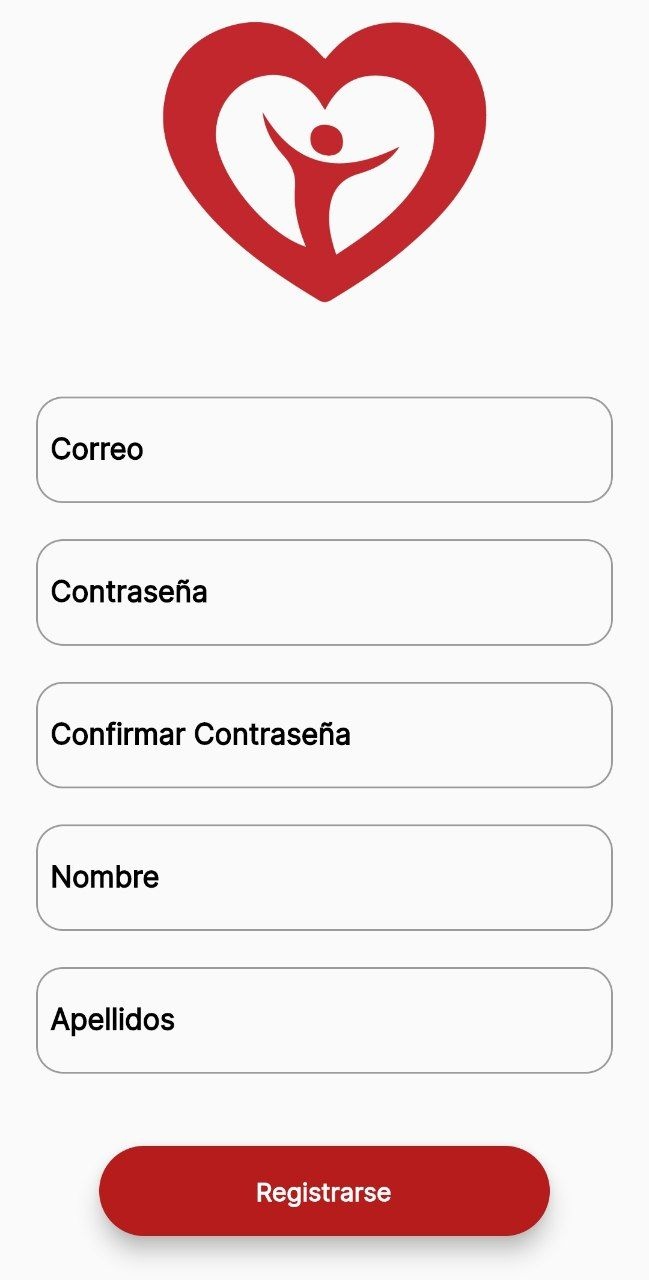
\includegraphics[scale = 0.1]{Images/register.jpg}}
\begin{small}
\caption{Página de Registro}
\end{small}
\end{center}
\end{column}

\begin{column}{0.25\textwidth}
\begin{center}

\fbox{
\includegraphics[scale = 0.1]{Images/login.jpg}}
\begin{small}
\caption{Página de Autenticación}
\end{small}
\end{center}
\end{column}

\end{columns}
\end{frame}




\begin{frame}
\frametitle{Aplicación}
Página principal de la aplicación
\begin{columns}
\begin{column}{0.25\textwidth}
\begin{center}

\fbox{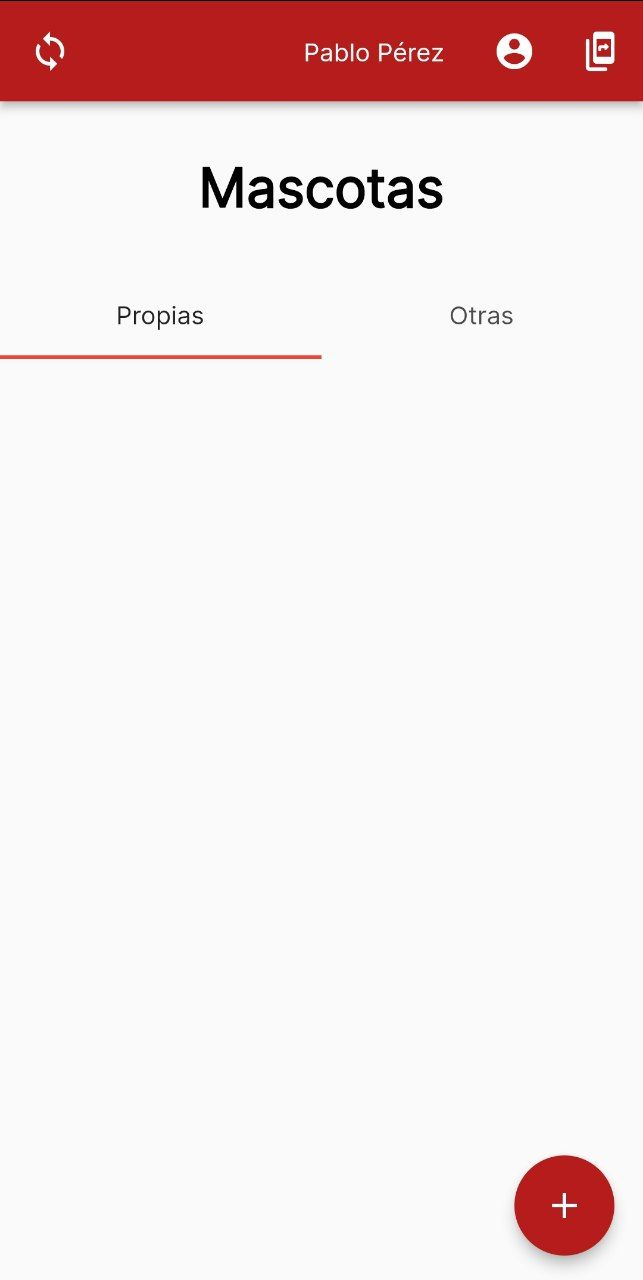
\includegraphics[scale = 0.1]{Images/home.jpg}}

\end{center}
\end{column}

\end{columns}
\end{frame}


\begin{frame}
\frametitle{Aplicación: Creación de Mascota}

\begin{columns}

\begin{column}{0.5\textwidth}
\begin{center}

\fbox{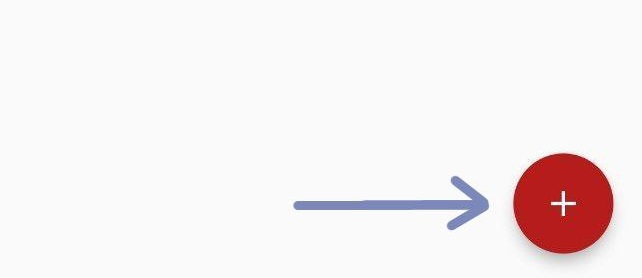
\includegraphics[scale = 0.16]{Images/createButt.jpg}}
\begin{small}


\caption{Botón de Crear Mascota}
\end{small}
\end{center}
\end{column}



\begin{column}{0.5\textwidth}
\begin{center}

\fbox{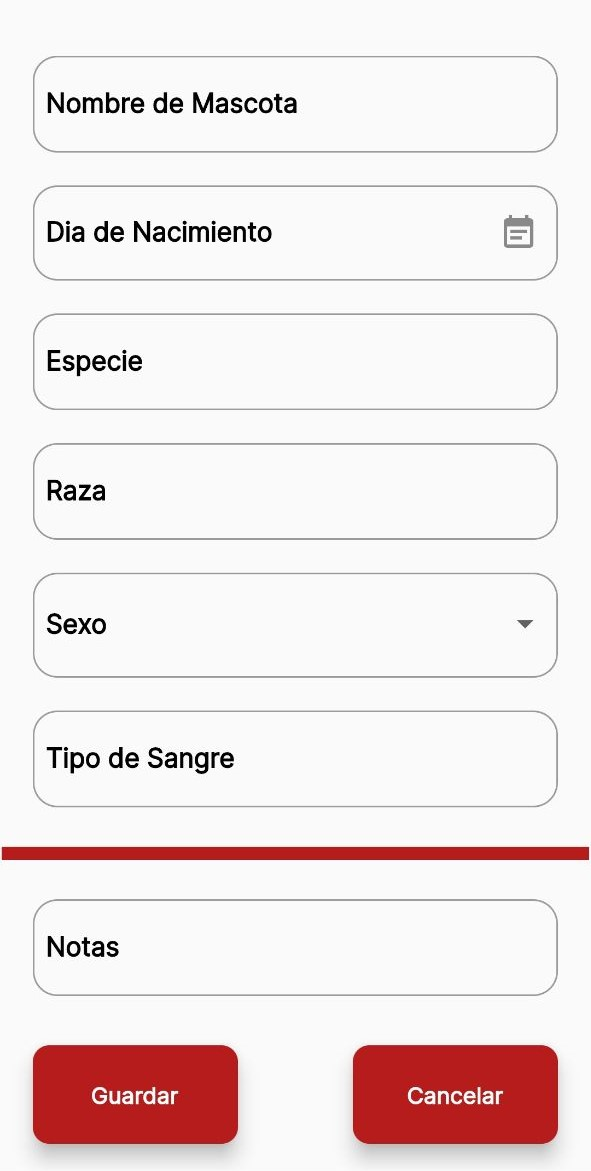
\includegraphics[scale = 0.16]{Images/createPet.jpg}}
\begin{small}



\caption{Página de Creación de Mascotas}
\end{small}
\end{center}
\end{column}

\end{columns}

\end{frame}


\begin{frame}
\frametitle{Aplicación}
Página principal de la aplicación con una mascota
\begin{columns}
\begin{column}{0.25\textwidth}
\begin{center}

\fbox{
\includegraphics[scale = 0.12]{Images/homePage.jpg}}

\end{center}
\end{column}

\end{columns}

\end{frame}


\begin{frame}
\frametitle{Aplicación: Eliminación}


\begin{columns}
\begin{column}{0.3\textwidth}
\begin{center}

\fbox{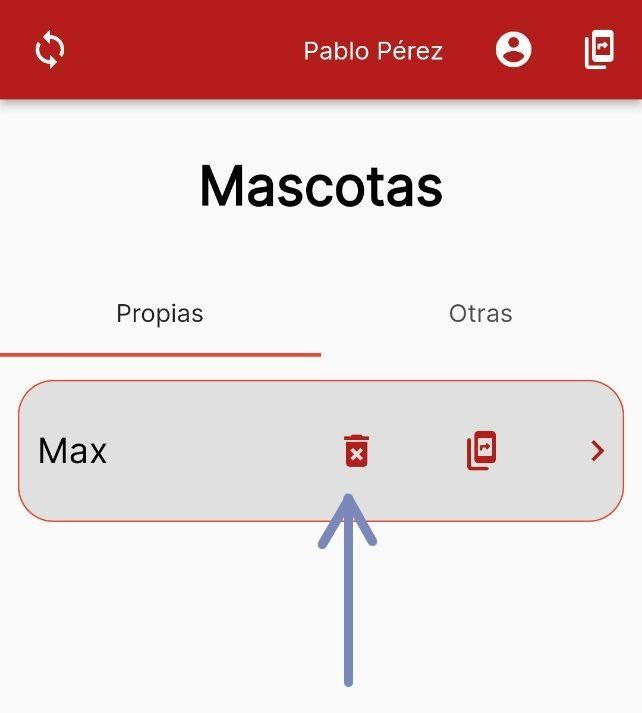
\includegraphics[scale = 0.12]{Images/deleteButt.jpg}}
\begin{small}
\caption{Botón para eliminar mascota}
\end{small}
\end{center}
\end{column}


\begin{column}{0.3\textwidth}
\begin{center}

\fbox{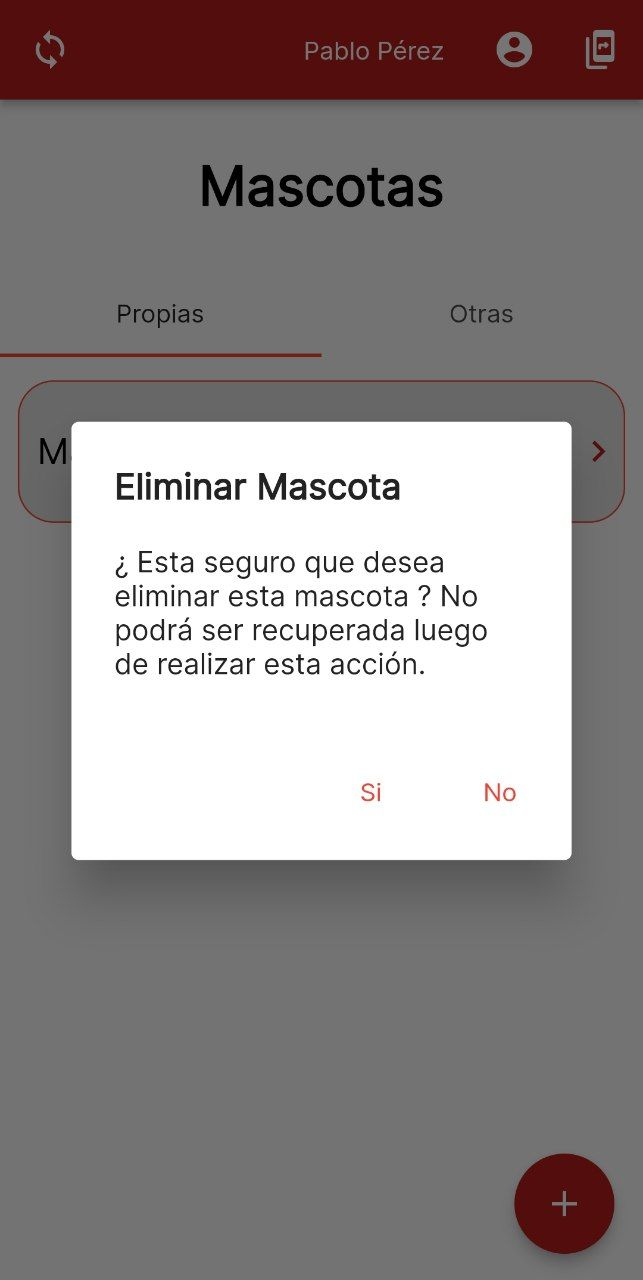
\includegraphics[scale = 0.12]{Images/deleteWarning.jpg}}
\begin{small}
\caption{Advertencia sobre la eliminación}
\end{small}
\end{center}
\end{column}

\end{columns}

\end{frame}






\begin{frame}
\frametitle{Aplicación: Creación de Consultas}

\begin{columns}

\begin{column}{0.3\textwidth}
\begin{center}

\fbox{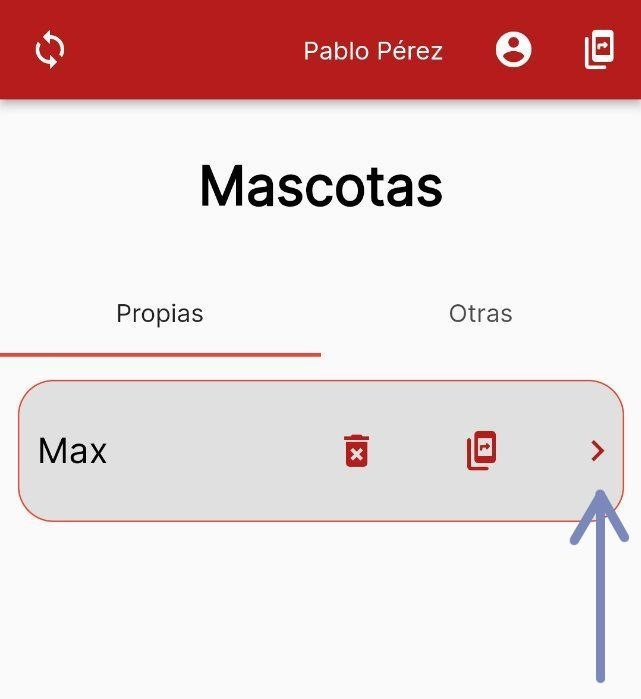
\includegraphics[scale = 0.1]{Images/formButt.jpg}}
\begin{small}
\caption{Botón para acceder a los formularios}
\end{small}
\end{center}
\end{column}


\begin{column}{0.3\textwidth}
\begin{center}

\fbox{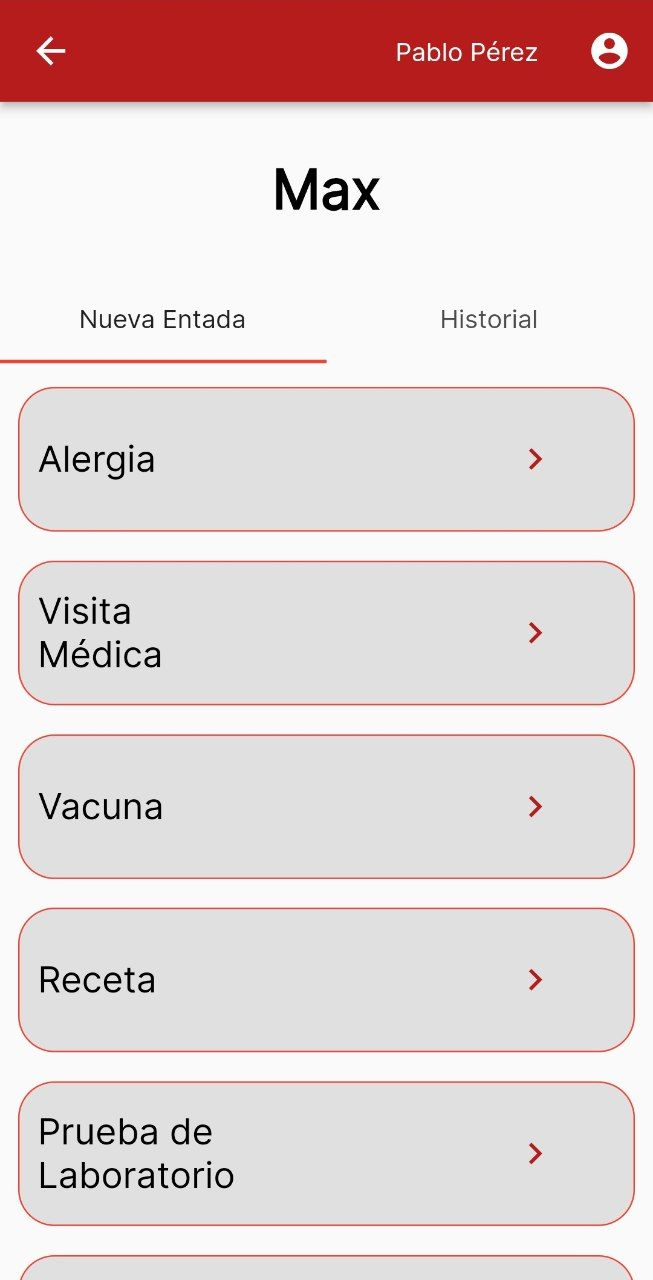
\includegraphics[scale = 0.1]{Images/addForm.jpg}}
\begin{small}
\caption{Página de Formularios}
\end{small}
\end{center}
\end{column}

\begin{column}{0.3\textwidth}
\begin{center}

\fbox{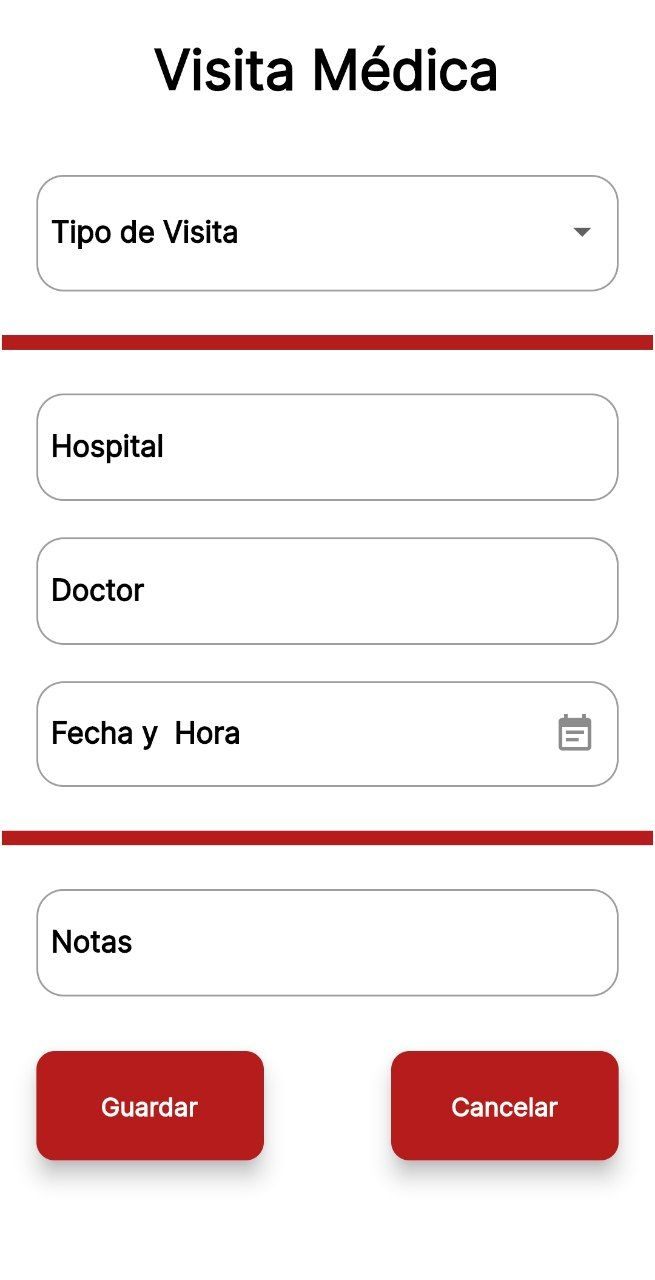
\includegraphics[scale = 0.1]{Images/MedVis.jpg}}
\begin{small}
\caption{Formulario de Visita Médica}
\end{small}
\end{center}
\end{column}

\end{columns}
\end{frame}


\begin{frame}
\frametitle{Aplicación: Historial Clínico}

\begin{columns}
\begin{column}{0.3\textwidth}
\begin{center}

\fbox{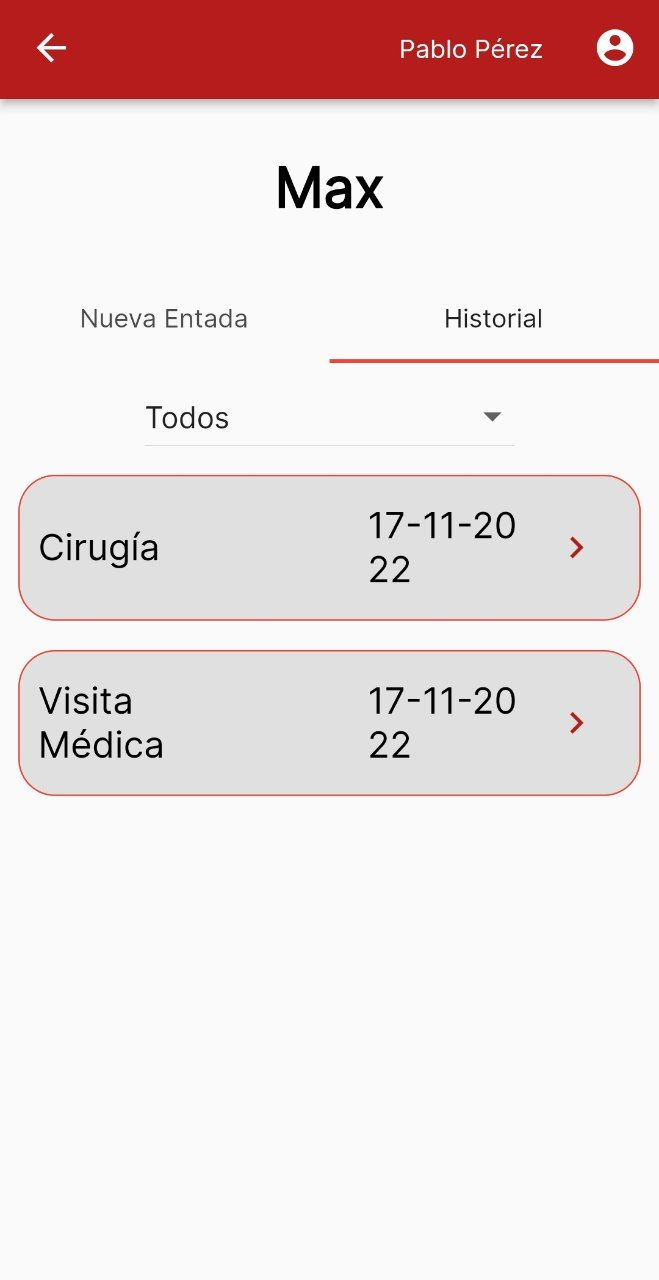
\includegraphics[scale = 0.1]{Images/hc.jpg}}
\begin{small}
\caption{Historia Clínica de la Mascota}
\end{small}
\end{center}
\end{column}

\begin{column}{0.3\textwidth}
\begin{center}

\fbox{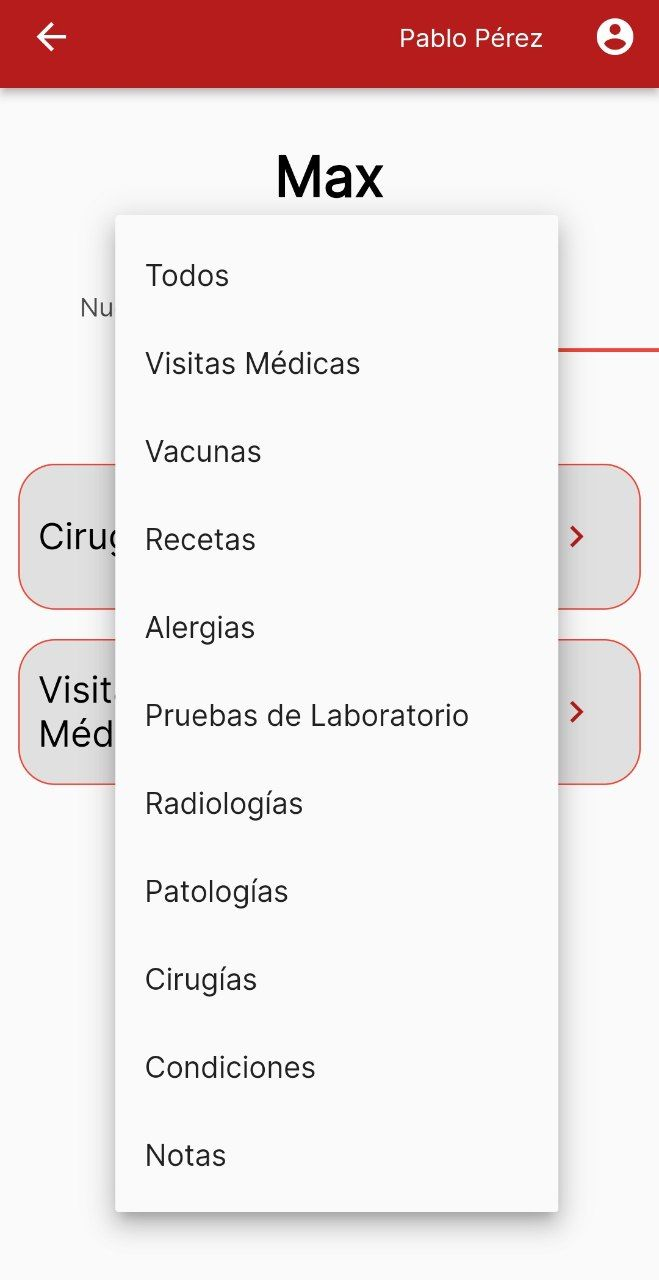
\includegraphics[scale = 0.1]{Images/selecthc.jpg}}
\begin{small}
\caption{Selección del tipo de formulario}
\end{small}
\end{center}
\end{column}

\end{columns}
\end{frame}


\begin{frame}
\frametitle{Aplicación: Consulta}
Muestra de una consulta de Visita Médica
\begin{columns}
\begin{column}{0.3\textwidth}
\begin{center}

\fbox{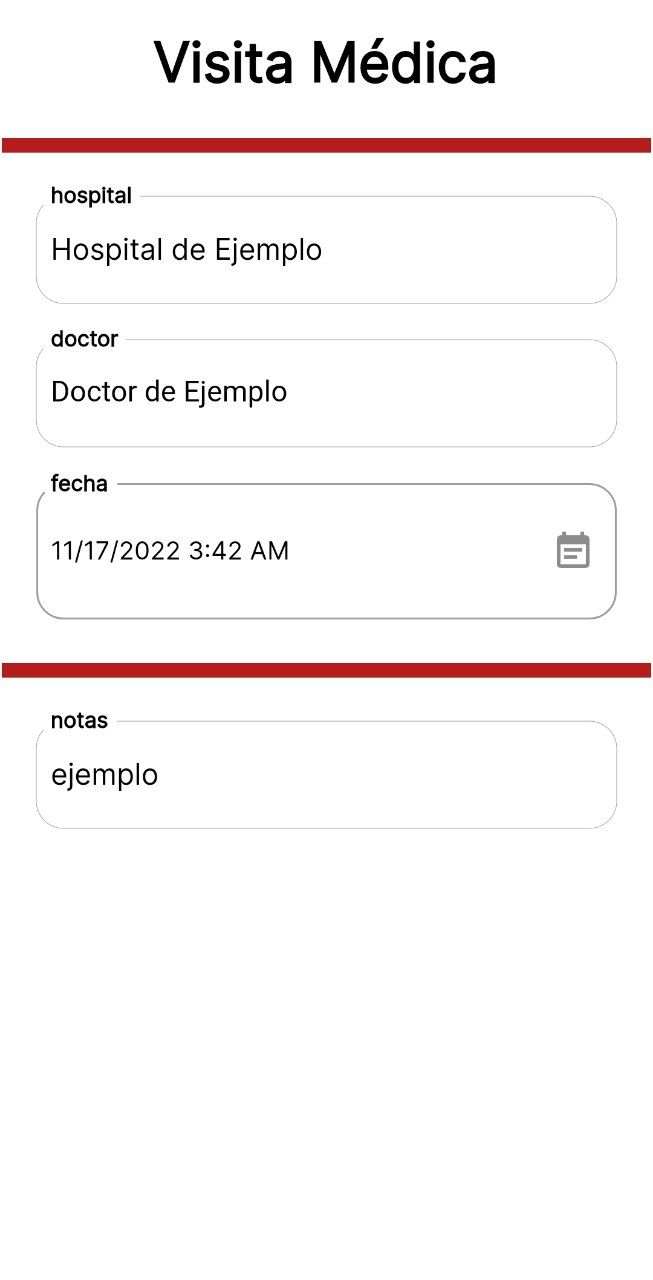
\includegraphics[scale = 0.1]{Images/medVshow.jpg}}
\begin{small}
\caption{}
\end{small}
\end{center}
\end{column}


\end{columns}

\end{frame}



\begin{frame}
\frametitle{Aplicación: Exportación e Importación de Mascotas}
Botones de importación y exportación de mascota
\begin{columns}
\begin{column}{0.5\textwidth}
\begin{center}

\fbox{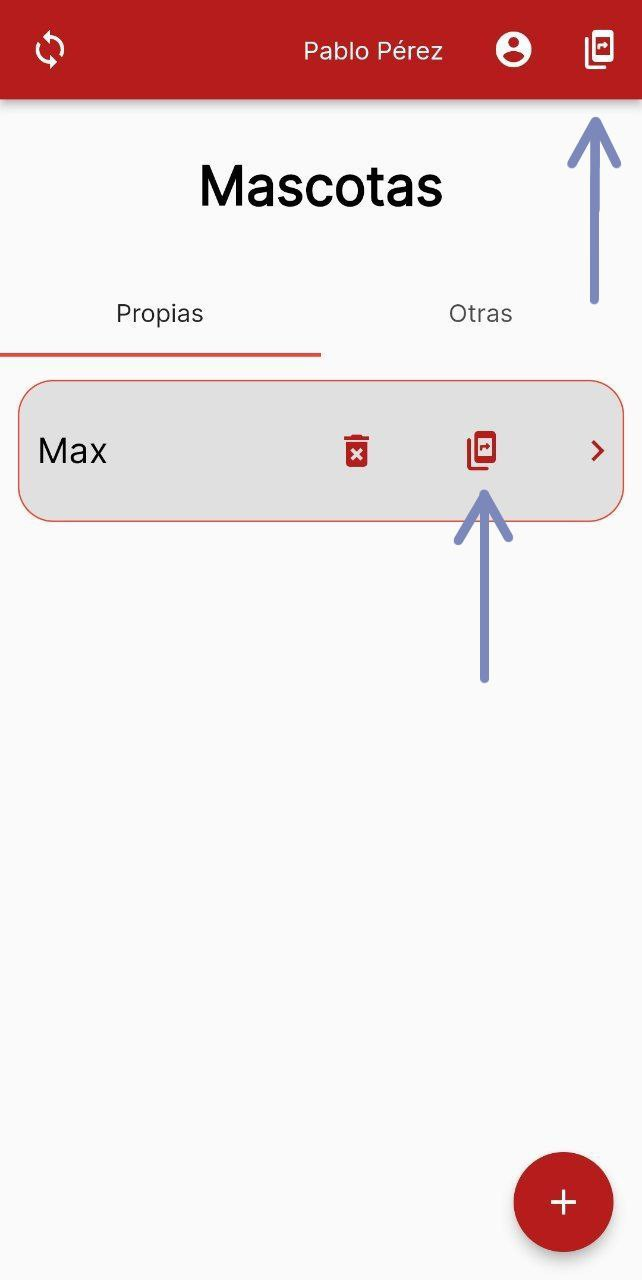
\includegraphics[scale = 0.12]{Images/homeA1.jpg}}

\end{center}
\end{column}

\end{columns}

\end{frame}





\begin{frame}
\frametitle{Aplicación: Exportación e Importación de Mascotas}
\begin{columns}
\begin{column}{0.3\textwidth}
\begin{center}

\fbox{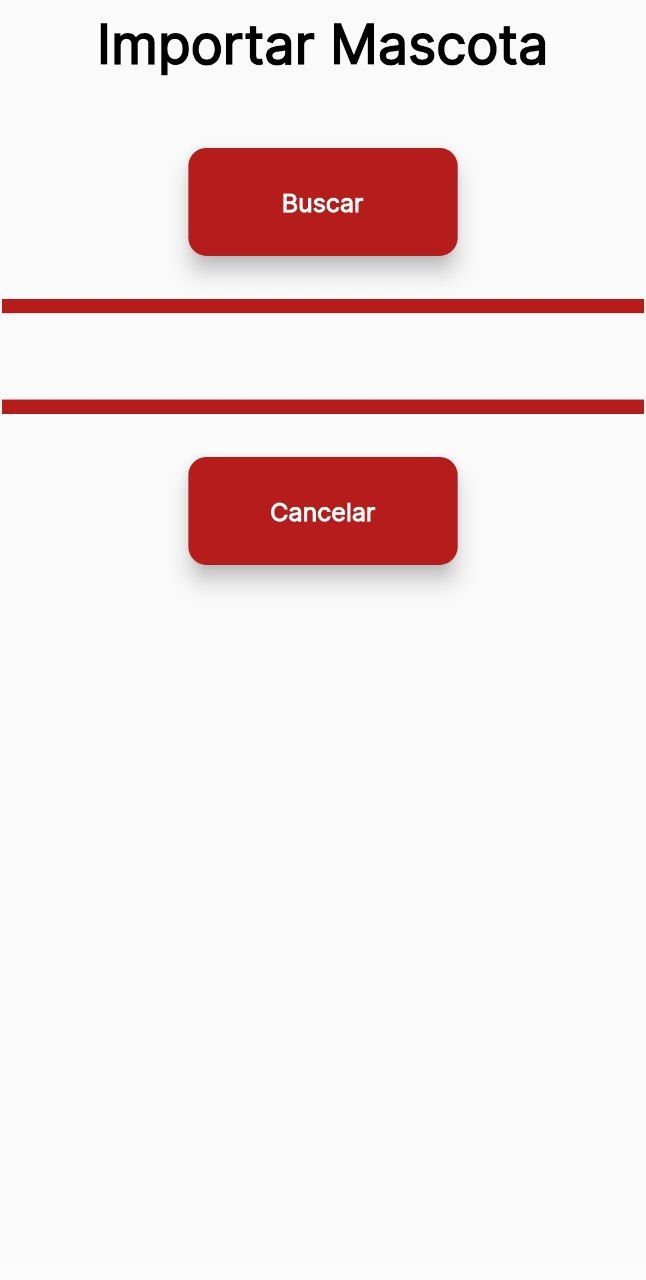
\includegraphics[scale = 0.1]{Images/import.jpg}}
\begin{small}
\caption{Página de Importación}
\end{small}
\end{center}
\end{column}

\begin{column}{0.3\textwidth}
\begin{center}

\fbox{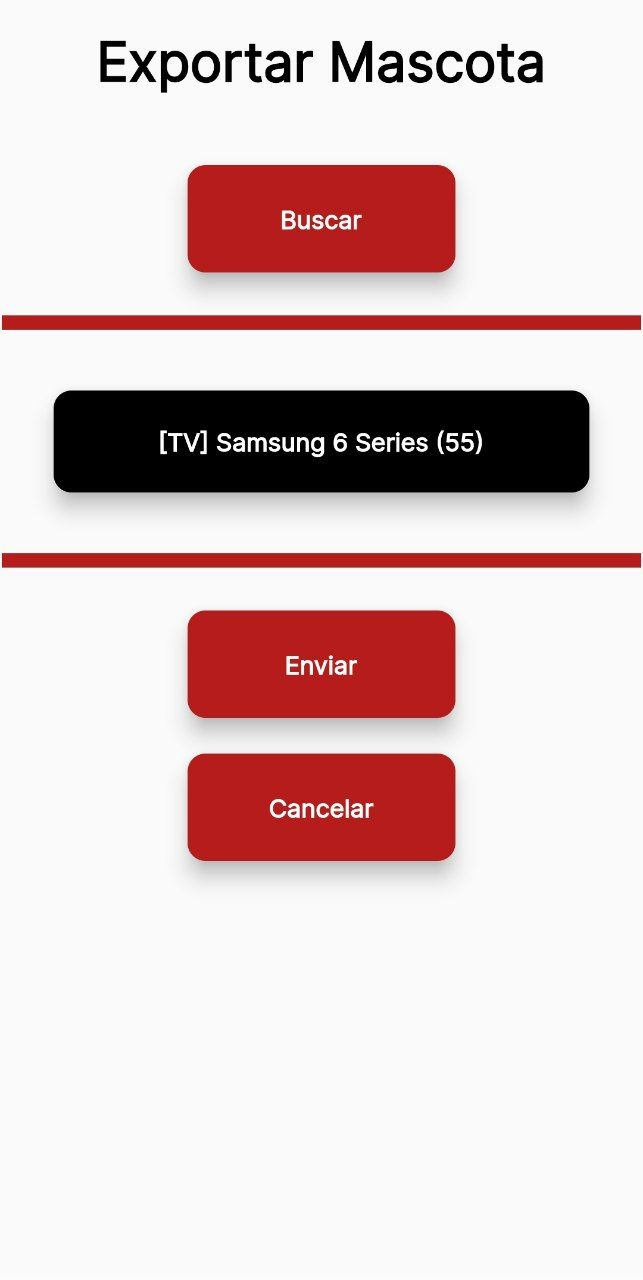
\includegraphics[scale = 0.1]{Images/exportdevice.jpg}}
\begin{small}
\caption{Página de Exportación}
\end{small}

\end{center}
\end{column}

\end{columns}
\end{frame}



\begin{frame}
\frametitle{Aplicación: Sincronización}

\begin{columns}

\begin{column}{0.5\textwidth}
\begin{center}

\fbox{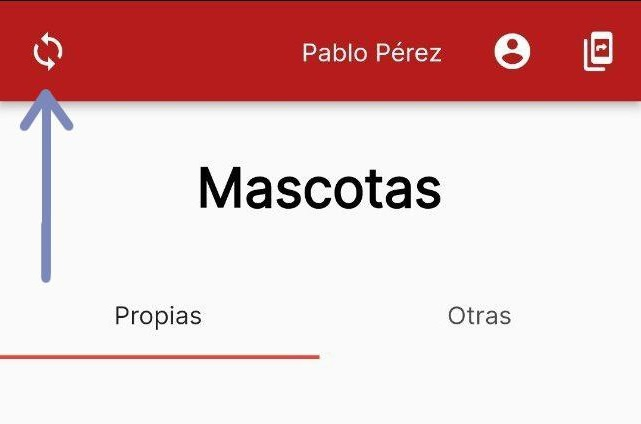
\includegraphics[scale = 0.2]{Images/synButt.jpg}}
\begin{small}
\caption{Botón de Sincronización Manual}
\end{small}
\end{center}
\end{column}


\begin{column}{0.5\textwidth}
\begin{center}

\fbox{
\includegraphics[scale = 0.17]{Images/synchro.jpg}}
\begin{small}
\caption{Mensaje de Sincronización Exitosa}
\end{small}
\end{center}
\end{column}


\end{columns}

\end{frame}



\begin{frame}
\frametitle{Conclusiones}
\begin{itemize}
\item[\checkmark] Se investigaron los requerimientos de las historias clínicas veterinarias.
\item[\checkmark] Fue realizado un estudio sobre aplicaciones móviles existentes.
\item[\checkmark] Se investigaron diferentes tecnologías de desarrollo.
\item[\checkmark] La aplicación cumple con los objetivos planteados.
\end{itemize}
\end{frame}



\begin{frame}
\frametitle{Recomendaciones}

\begin{itemize}
\item Otros tipos de consultas.
\item Modificar datos.
\item Sistema de citas controlado por el servidor.
\item Diferenciar entre distintos tipos de usuarios.
\item Sistema de avisos y alarmas.
\end{itemize}

\end{frame}





\begin{frame}
\maketitle
\end{frame}




\begin{frame}
\frametitle{Primera pregunta del oponente}
\begin{block}{Pregunta 1}
 Una de ls tareas planteadas en la Tesis dice ''Analizar y probar tecnologías de desarrollo de aplicaciones móviles y bases de datos que permitan el rápido desarrollo del producto deseado''. Sin embargo, un poco antes, al plantear las hipótesis, escriben ''Trabajando sobre la plataforma Flutter a través de Dart''. Aparentemente hay una contradicción entre la tarea de analizar y probar diversas tecnologías y la selección a priori de UNA tecnología concreta para el desarrollo en las hipótesis del trabajo. ¿Podrían comentar al respecto?
\end{block}
\end{frame}


\begin{frame}
\frametitle{Primera pregunta del oponente}
\begin{block}{Hipótesis}
"...sobre la plataforma Flutter a través de Dart, es posible crear un interfaz de usuario funcional..."
\end{block}

\begin{alertblock}{Tareas}
\begin{itemize}
\item ''Analizar y probar tecnologías de desarrollo de aplicaciones móviles ..."
\end{itemize}

\end{alertblock}
\end{frame}

\begin{frame}
\frametitle{Tecnologías analizadas}
\begin{itemize}
\item Java
\item Kotlin
\item Xamarin
\item React Native
\item \textbf{Flutter}

\end{itemize}

\end{frame}






\begin{frame}
\frametitle{Ventajas de Flutter}

\begin{itemize}
\item Representación en todas las plataformas.
\item Funcionalidad de Hot Reload.
\item Fácil diseño de interfaz gráfica.
\item Documentación completa y de calidad.
\item Es Open-Source.
\end{itemize}

\end{frame}










\begin{frame}
\frametitle{Segunda pregunta del oponente}
\begin{block}{Pregunta 2}
De todos es conocido que los profesionales de la salud, e imagino que en el caso de la salud animal de cierta forma esté también presente, es muy importante el ''ojo clínico'', la visualización del paciente, no solamente los datos alfanumérifcos asociados a una HC tradicinal. ¿Han considerado la idea de incluir fotos e inlcuso videos del comportamiento del animal como parte de la historia, pensando en futuras comparaciones visuales por parte de los profesionales al consultarlos?
\end{block}
\end{frame}



\begin{frame}
\frametitle{Primeros diseños de la aplicaión(7/2022)}


\begin{columns}
\begin{column}{0.5\textwidth}
\begin{center}

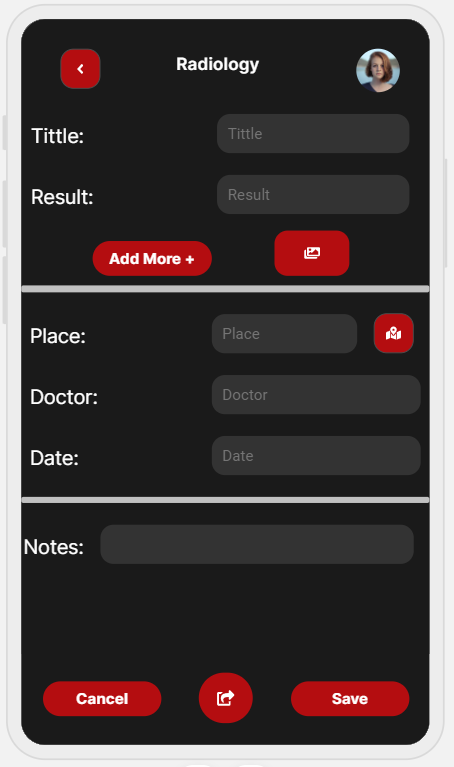
\includegraphics[scale = 0.35]{Images/photoExample.png}

\end{center}
\end{column}
\begin{column}{0.5\textwidth}
\begin{center}

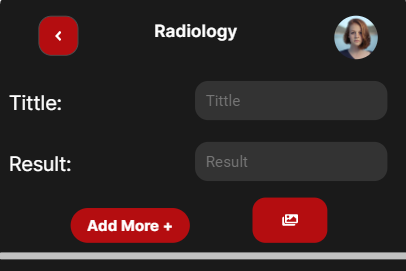
\includegraphics[scale = 0.55]{Images/photoExampleZoom.png}

\end{center}
\end{column}
\end{columns}

\end{frame}


\begin{frame}
\frametitle{Con respecto al almacenamiento interno.}
Tipos de datos soportados por SQLite:
\begin{itemize}
\item Integer
\item Real
\item Text
\item BLOB
\end{itemize}

\end{frame}


\begin{frame}
\frametitle{Con respecto al almacenamiento interno.}
Tipos de datos soportados por SQLite:
\begin{itemize}
\item Integer
\item Real
\item Text
\item BLOB
\end{itemize}

\end{frame}

\begin{frame}
\frametitle{Transmisión de Datos}
Problemas:
\begin{itemize}
\item Almacenamiento de imágenes en el servidor.
\item Sincronización de imágenes en dispositivos
\item Envío de mascotas de manera local
\end{itemize}


\end{frame}
\begin{frame}
\frametitle{Guardar imágenes}
Biblioteca:\textbf{image\_picker}(Pub.dev)
\begin{columns}
\begin{column}{0.5\textwidth}
\begin{center}

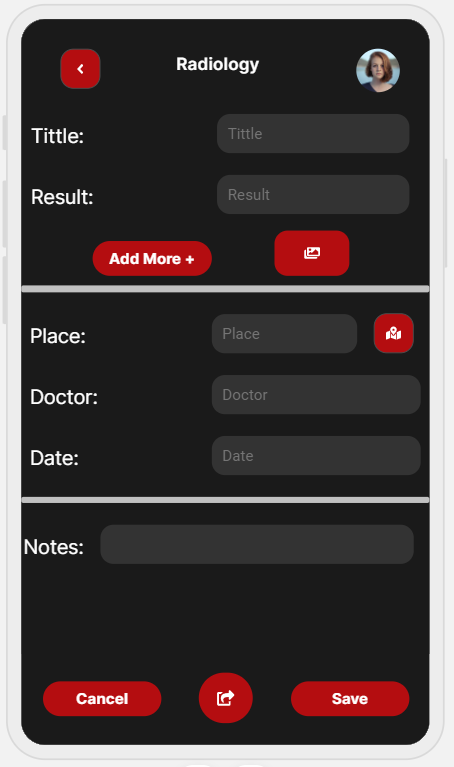
\includegraphics[scale = 0.32]{Images/photoExample.png}

\end{center}
\end{column}
\begin{column}{0.5\textwidth}
\begin{center}

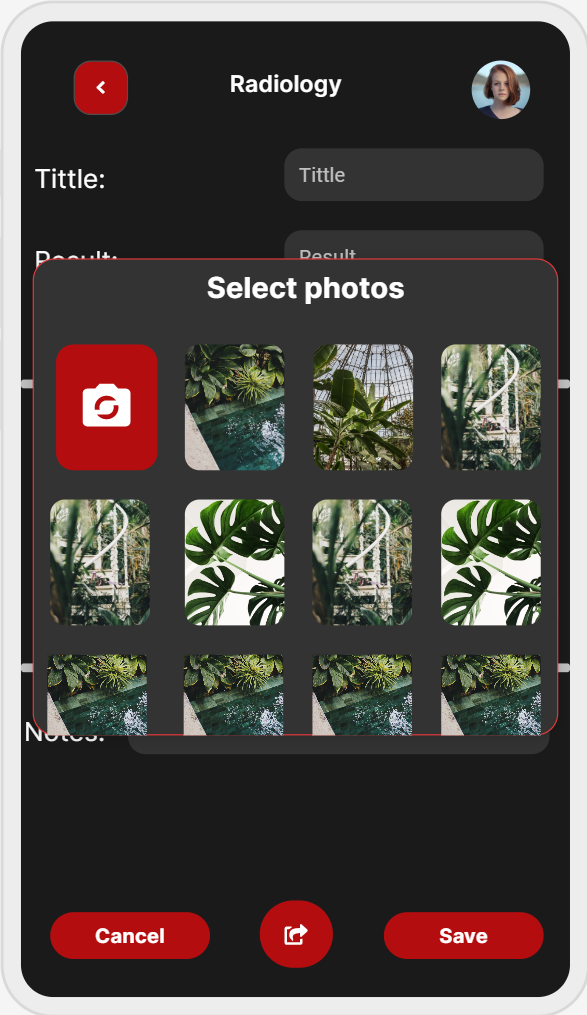
\includegraphics[scale = 0.48]{Images/RadiologyP.png}

\end{center}
\end{column}
\end{columns}


\end{frame}

\begin{frame}
\frametitle{Cargar imágenes}
Biblioteca:\textbf{image\_picker}(Pub.dev)
\begin{columns}
\begin{column}{0.5\textwidth}
\begin{center}

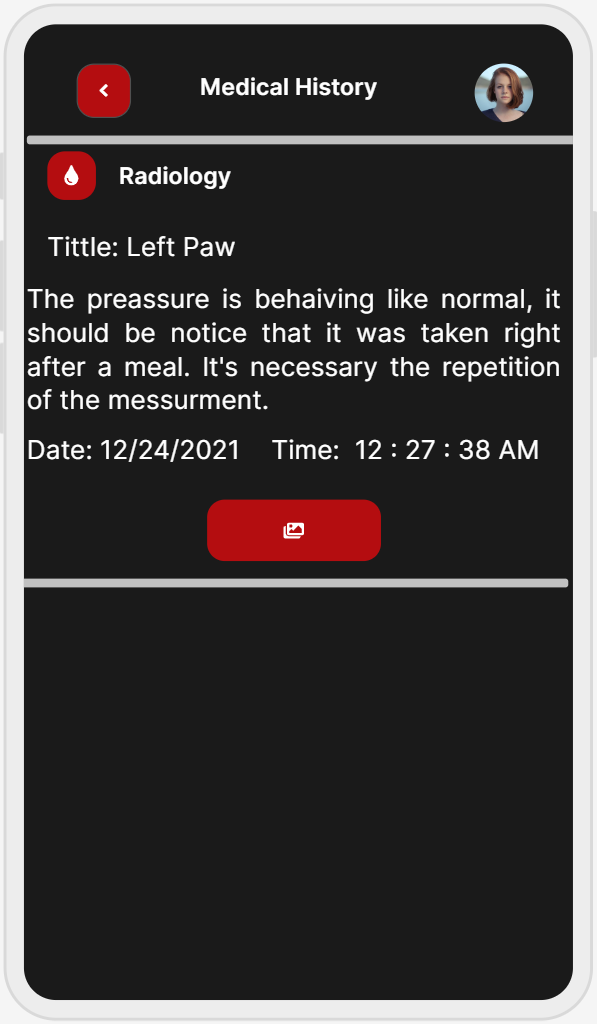
\includegraphics[scale = 0.48]{Images/History.PNG}

\end{center}
\end{column}
\begin{column}{0.5\textwidth}
\begin{center}

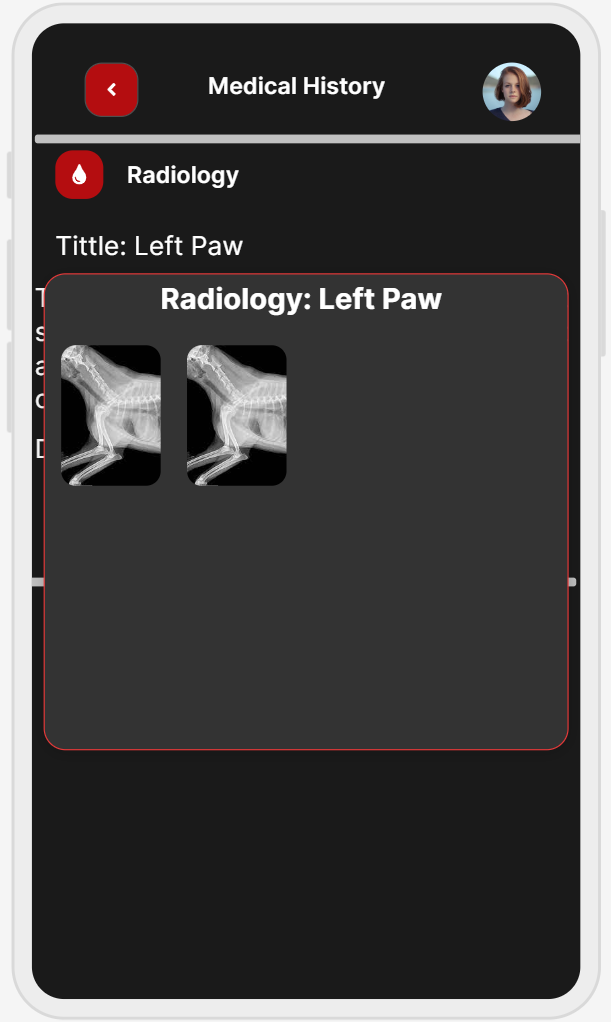
\includegraphics[scale = 0.48]{Images/HistoryP.PNG}

\end{center}
\end{column}
\end{columns}


\end{frame}




\end{document}